\documentclass[a4paper, 1.5lines]{ctexart}
\usepackage[top=3cm, bottom=2cm]{geometry}
\usepackage{graphicx}
\usepackage{subcaption}
\usepackage{amsmath}
\usepackage{xcolor}
\usepackage{url}
%\usepackage{hyperref}
\usepackage[hidelinks]{hyperref} % 加载 hyperref 并隐藏链接边框

%\usepackage[utf8]{inputenc}
%\usepackage[ngerman]{babel} % 加载德语支持

% booktabs 提供 \toprule, \midrule, \bottomrule 等表格命令
\usepackage{booktabs}
% 定义占位命令以避免未定义控制序列错误
\newcommand{\placeholderspace}{}
\usepackage{fancyhdr} % 导入fancyhdr宏包
\usepackage{lipsum}   % 仅用于生成示例文本
\usepackage{float}    % 提供 H 浮动位置选项

% 设置页面样式为fancy
\pagestyle{fancy}
% 自定义页眉内容
\fancyhead[L]{} % 左侧页眉
\fancyhead[C]{\textbf{Physics-experiment Reporting Letter:\\Properties of High-Temperature Superconducting Materials}} % 中间页眉
\fancyhead[R]{ } % 右侧页眉
% 自定义页脚内容
\fancyfoot[L]{ } % 左侧页脚
\fancyfoot[C]{\thepage} % 中间页脚显示页码
\fancyfoot[R]{ } % 右侧页脚
% 改变页眉线的粗细
\renewcommand{\headrulewidth}{1.4pt}
% 改变页脚线的粗细
\renewcommand{\footrulewidth}{0.pt}





\title{高温超导材料的特性与表征实验报告}
\author{实验人：唐亿\qquad 学号：202311998381\qquad 指导教师：张金星}
\date{实验日期：2025.10.10}


\begin{document}
    
    \maketitle
    
    \begin{abstract}
          本实验旨在研究高温超导材料 $\text{YBa}_2\text{Cu}_3\text{O}_{7-\delta}$ 的基本电磁特性，包括完全导电性和完全抗磁性（迈斯纳效应），并精确测定其临界转变温度 ($T_c$)。
          实验方法分为两部分：一是使用液氮冷却样品，并利用永磁体定性观察磁悬浮现象，验证迈斯纳效应；二是通过四端法测量样品在冷却过程中的电阻-温度 ($R-T$) 曲线。通过 $R-T$ 曲线，计算电阻突降至零时的临界温度。
          实验结果证实了高温超导体在液氮温区表现出显著的完全抗磁性，且 $R-T$ 曲线显示出明确的超导转变，测得临界温度 $T_c \approx 94\text{K}$。
          本次实验成功表征了 $\text{YBa}_2\text{Cu}_3\text{O}_{7-\delta}$ 的超导特性，加深了对宏观量子现象的理解。

          \textbf{关键词：} 高温超导；迈斯纳效应；临界温度；$\text{YBa}_2\text{Cu}_3\text{O}_{7-\delta}$
    \end{abstract}
    
    \section{引言}
        \label{sec:introduction}

        \subsection{实验背景与发展历程}
        超导电性是凝聚态物理学中的一个重要现象。它始于 1911 年，昂内斯（H.K. Onnes）发现汞在 4.2 K 时电阻突然消失。随后，迈斯纳（W. Meissner）在 1933 年发现了超导体的另一个基本特性——完全抗磁性，即迈斯纳效应。这一发现确立了超导态是一种真正的热力学态。超导研究的重大突破发生在 1986 年，柏诺兹（J.G. Bednorz）和缪勒（K.A. Müller）发现了临界温度 ($T_c$) 超过 30 K 的铜氧化物陶瓷材料，开创了高温超导（High-$T_c$ Superconductivity）的新纪元。这些高温超导材料，例如本实验所用的 $\text{YBa}_2\text{Cu}_3\text{O}_{7-\delta}$ (YBCO)，其 $T_c$ 超过了液氮的沸点（77 K），极大地降低了超导应用所需的制冷成本。

        \subsection{应用前景与实验目的}
        超导技术因其零电阻和完全抗磁性，在磁悬浮列车、超导量子干涉仪（SQUID）、高能物理中的超导磁体以及未来的核磁共振（MRI）等领域具有广阔的应用前景。本实验旨在通过对高温超导材料的基本特性进行表征，加深对超导现象的理解。具体实验目的如下：
        \begin{enumerate}
            \item 了解超导电性的发展历程、基本概念和高温超导体的特性。
            \item 通过液氮冷却和永磁体，定性观察高温超导体的迈斯纳效应（完全抗磁性）。
            \item 掌握四端法测量电阻的技术，精确测定 $\text{YBa}_2\text{Cu}_3\text{O}_{7-\delta}$ 的临界转变温度 ($T_c$)。
        \end{enumerate}

    \section{原理}
        \label{sec:principle}

        \subsection{超导体的两大基本特性}
        超导态是一种宏观量子现象，由两个核心特性定义：
            \subsubsection{完全导电性（Zero Resistance）}
            当温度 $T$ 低于临界温度 $T_c$ 时，材料的直流电阻 $\rho$ 突降至零。这意味着超导体可以承载无损耗的电流。
            \subsubsection{完全抗磁性（Meissner Effect）}
            当材料从正常态冷却进入超导态时，其内部的磁通量被完全排斥出体外（$B=0$）。迈斯纳效应揭示了超导态是一个热力学稳定态，而非简单电阻消失的理想导体。这种效应是本实验中磁悬浮现象的物理基础。
        

        \begin{figure}[H]
        \centering    
        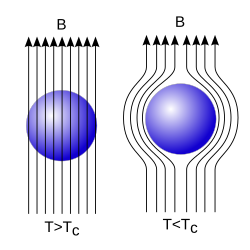
\includegraphics[width=0.4\textwidth]{fig//EfektMeisnera.svg.png} 
        \caption{迈斯纳效应示意图}
        \label{fig:meissner_principle}
        \end{figure}

        \subsection{临界参数：临界温度 ($T_c$) 与临界磁场 ($H_c$)}
        超导电性并非在任何条件下都能维持，它受到三个参数的共同限制：温度 ($T$)、磁场 ($H$) 和电流密度 ($J$)。当其中任一参数超过其临界值，超导体就会从超导态（S态）转变为正常态（N态）。
        \begin{itemize}
            \item 临界温度 ($T_c$)：在零磁场和零电流下，超导转变发生的温度。
            \item 临界磁场 ($H_c$)：在给定温度下，能够破坏超导态所需的最小外加磁场强度。 $H_c$ 随温度降低而增大。
        \end{itemize}

        \subsection{第一类和第二类超导体}
        根据对磁场的响应特性，超导体可分为两类：
            \subsubsection{第一类超导体（软超导体）}
            它们完全遵循迈斯纳效应，磁场一旦达到临界磁场 $H_c$，材料便立即从完全抗磁的超导态转变为正常态。它们通常具有较低的 $T_c$ 和 $H_c$。
            \subsubsection{第二类超导体（硬超导体）}
            所有高温超导体（包括本实验的 $\text{YBa}_2\text{Cu}_3\text{O}_{7-\delta}$）均属于第二类。它们有两个临界磁场：
            \begin{enumerate}
                \item 下临界磁场 ($H_{c1}$)：在 $H < H_{c1}$ 时，材料处于完全迈斯纳态 ($B=0$)。
                \item 上临界磁场 ($H_{c2}$)：在 $H_{c1} < H < H_{c2}$ 时，材料进入混合态（或涡旋态）。此时磁通线以量子涡旋的形式穿透样品，但大部分材料仍保持超导。只有当 $H > H_{c2}$ 时，超导性才彻底消失，转变为正常态。
            \end{enumerate}
            第二类超导体拥有更高的 $H_{c2}$，使其在高场应用中具有巨大价值。

            \begin{figure}[H]
                \centering    
                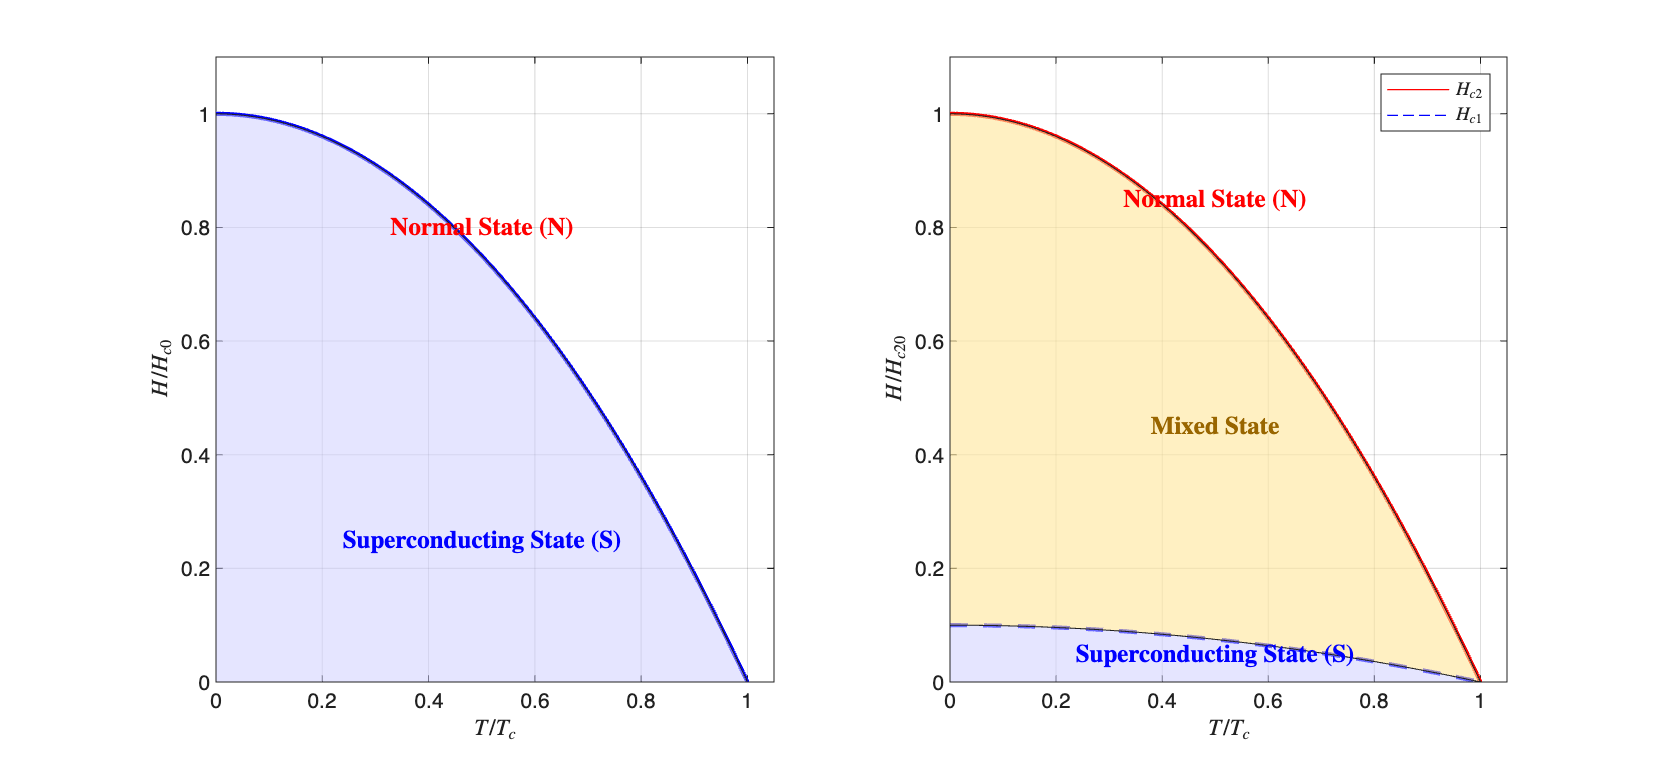
\includegraphics[width=1.2\textwidth]{fig//Superconductor H-T Phase Diagram Comparison (Normalized).png} 
                \caption{两类超导体的$H-T$示意图(左:第一类;右:第二类)}
                \label{fig:meissner_principle}
            \end{figure}

        \subsection{临界温度测量原理（四端法）}
        临界温度 $T_c$ 是超导体从正常态转变为超导态的温度。精确测量 $T_c$ 采用四端法（Four-probe method），其核心思想是消除测量过程中引线电阻和样品与电极之间的接触电阻带来的干扰。
        \begin{itemize}
            \item 电流端（外侧）： 通过两根引线施加恒定测量电流 $I$。
            \item 电压端（内侧）： 通过另外两根引线测量样品两端的电压降 $V$。
        \end{itemize}
        根据欧姆定律 $R = V/I$，计算出样品的真实电阻。当样品进入超导态后， $V \to 0$，即 $R \to 0$。通过监测 $R$ 随温度 $T$ 的变化 ($R-T$ 曲线)，可以确定电阻开始下降（$T_{c, \text{onset}}$）、中点（$T_{c, \text{mid}}$）和完全消失（$T_{c, \text{end}}$）的温度，从而准确表征 $T_c$。

    \newpage
    \section{实验}
       \label{sec:experiment} 
        \subsection{实验仪器}
        \subsubsection{高温超导样品}
            $\text{YBa}_2\text{Cu}_3\text{O}_{7-\delta}$ ($\text{YBCO}$)
        \subsubsection{液氮低温恒温系统}    
            本实验使用不锈钢杜瓦容器盛放液氮，通过将低温恒温容器放入杜瓦容器内实现低温温度的获得和控制。恒温器通过拉杆调整其在杜瓦瓶中的位置进而控制温度，拉杆固定螺母和夹子用于固定拉杆以防止恒温器滑动。
            紫铜圆筒起到均温作用，恒温器下方探出的螺钉需要伸到液氮中以实现热量交换。上、下挡板用于阻挡来自室温和液氮的辐射作用，液面计位于紫铜圆筒底部与下挡板间距离的 $\text{1/2}$ 处，用来监测恒温器与液氮表面距离的变化。
        \subsubsection{四引线电测量设备}
            \begin{itemize}
                \item 恒流源：提供稳定的直流小电流 $I$（例如 $\text{10 mA}$）。
                \item 高精度数字电压表：测量样品两电压探针间的微弱电压 $V$。
                \item 四引线连接装置：确保电流和电压测量探针独立连接，消除接触电阻影响。
            \end{itemize}
        \subsubsection{磁悬浮力测量设备}
            超导磁悬浮演示装置，包括 $\text{YBCO}$ 样品支架、永磁体以及配套的隔热保护装置。
            
        

        \subsection{实验方法}
            \subsubsection{温度扫描速率控制}
                在测量 $R-T$ 曲线时，精确的温度控制至关重要。通过恒温器拉杆调整样品与液氮液面距离进行调整。为了保证测量的准确性，尤其是在超导转变区（$T_\text{c}$ 附近），必须采用缓慢、稳定的降温。缓慢扫描有助于确保样品温度均匀，并使温度传感器与样品达到热平衡，从而更准确地确定临界温度 $T_\text{c}$ 和转变宽度 $\Delta T_\text{c}$。

            \subsubsection{零场冷（ZFC）与场冷（FC）}
                这两种冷却方式主要用于观察非完美超导体的磁通钉扎现象：
                \begin{enumerate}
                    \item \textbf{零场冷（Zero-Field Cooling, ZFC）}：\\
                    首先，在无外部磁场（$H=0$）的环境下，将超导样品从正常态（$T > T_\text{c}$）冷却至超导态（$T < T_\text{c}$）。

                    \item \textbf{场冷（Field Cooling, FC）}：\\
                    首先，将永磁体放置在超导样品附近（有外部磁场，$H \neq 0$），然后将整个系统从正常态冷却至超导态（$T < T_\text{c}$）。
                \end{enumerate}

    \section{结果与分析讨论}

        \subsection{$R-T$ 超导转变曲线绘制与临界温度确定}
        
        \begin{figure}[H]
            \centering    
            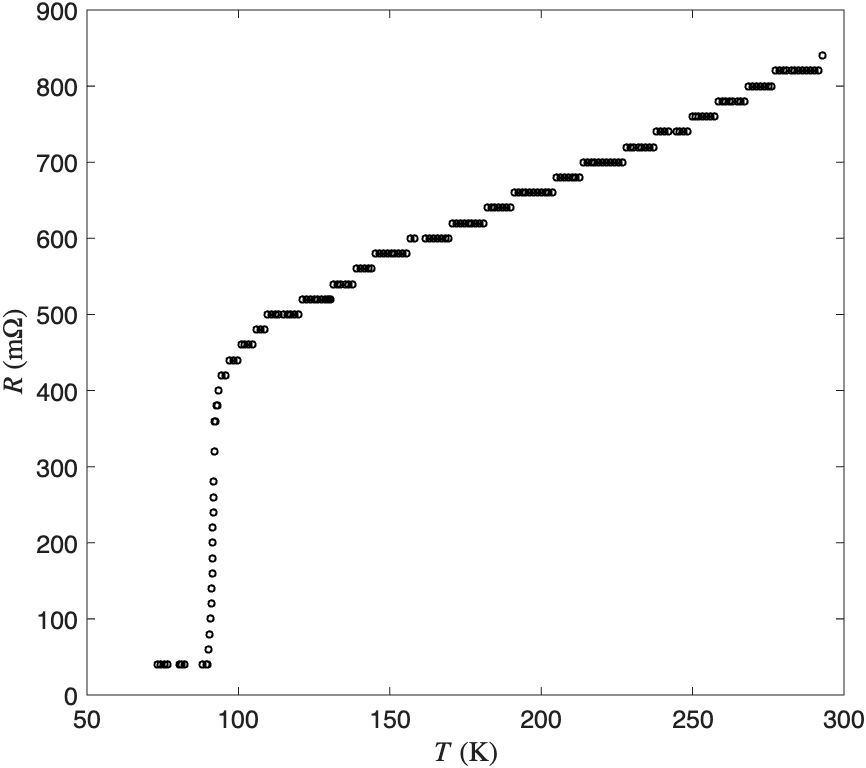
\includegraphics[width=0.6\textwidth]{fig//phase.png} 
            \caption{实验测得的 $R-T$ 超导转变曲线}
            \label{fig:RT_curve}
        \end{figure}

        我们对正常态的电阻温度曲线进行拟合,就能找到电阻开始下降的温度 $T_{c, \text{onset}}$。通过测量电阻降至零的温度 $T_{c, \text{end}}$，我们可以计算出超导转变宽度 $\Delta T_c = T_{c, \text{onset}} - T_{c, \text{end}}$。此外，取 $R$ 降至一半时的温度作为中点临界温度 $T_{c, \text{mid}}$。

        \begin{figure}[H]
            \centering    
            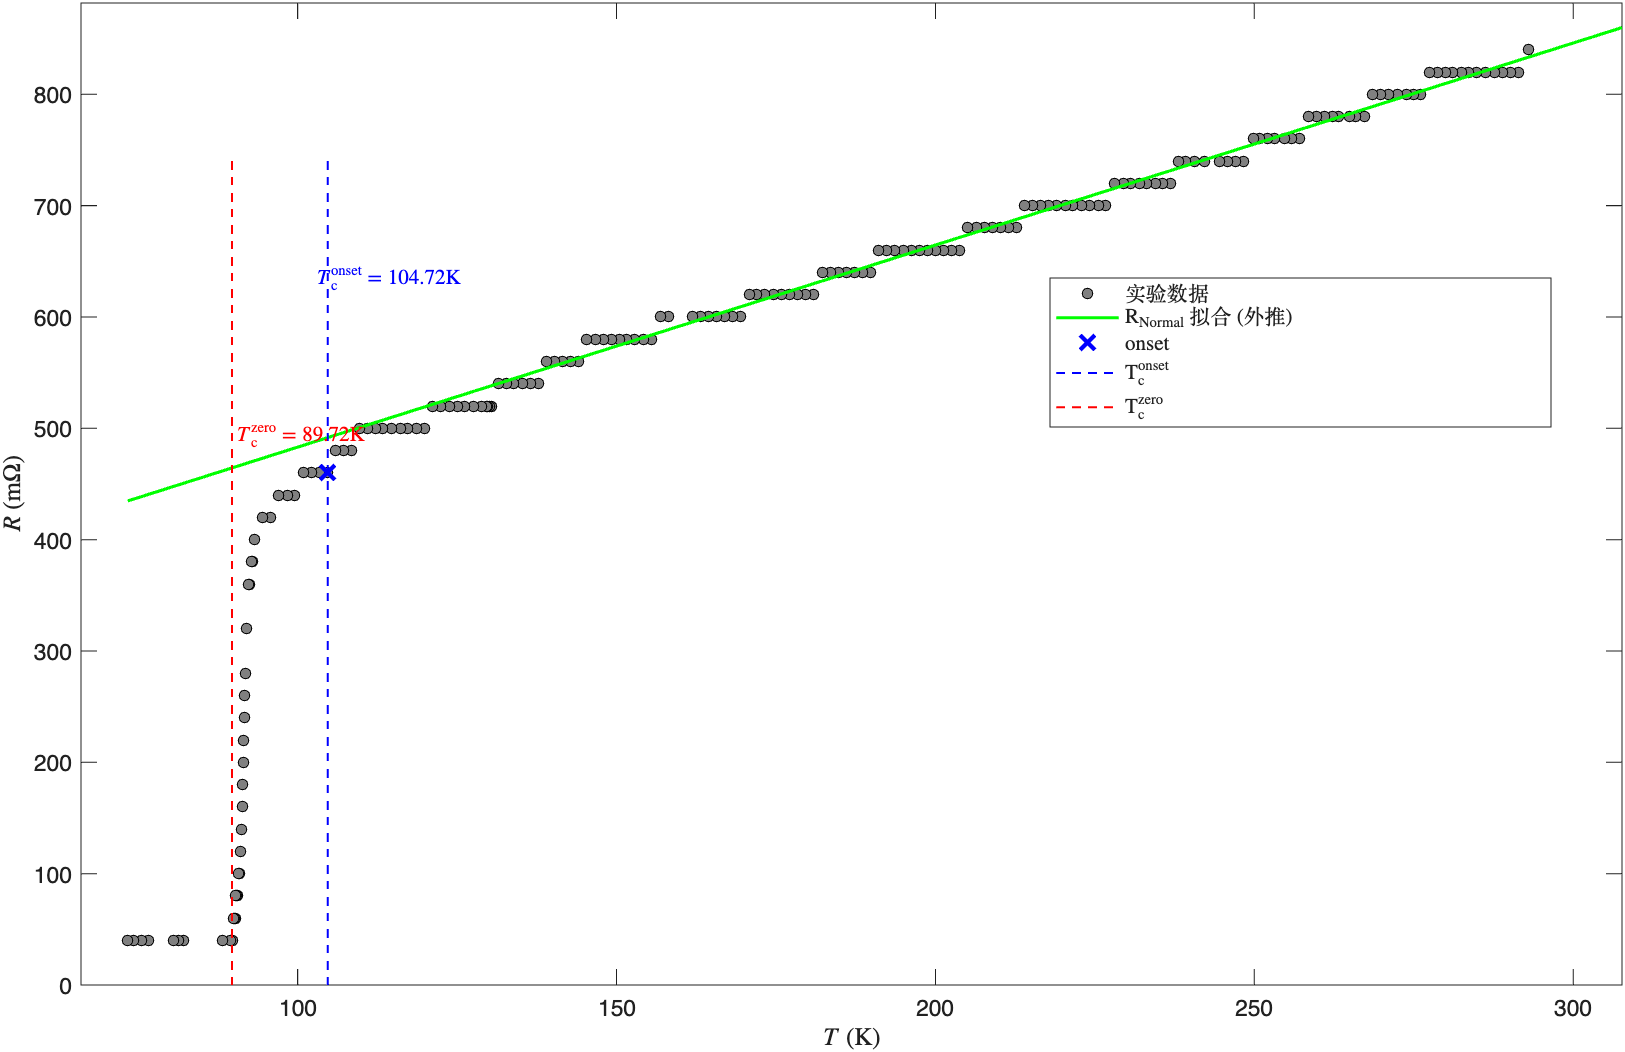
\includegraphics[width=0.8\textwidth]{fig//onset.png} 
            \caption{拟合得到转变温度}
            \label{fig:RT_curve_experiment}
        \end{figure}
        
        通过图中拟合曲线，我们得到以下结果：
        \begin{itemize}
            \item 起始临界温度 $T_{c, \text{onset}} \approx 104.72\text{K}$
            \item 中点临界温度 $T_{c} \approx 94 \text{K}$
            \item 结束临界温度 $T_{c, 0} \approx 89.72 \text{K}$
            \item 超导转变宽度 $\Delta T_c \approx 15 \text{K}$
        \end{itemize}

        \subsection{磁悬浮力测量}
            零场冷和场冷条件下磁悬浮力的测量结果分别如图(\ref{fig}a)、(\ref{fig}b)所示。在这两种情况下，都能观察到磁体靠近超导体和远离超导体的过程对应的受力情况存在差异，在图中显示为远离和靠近对应的受力-距离曲线并不重合。
    
    
            \subsubsection{ZFC}
            磁体先“靠近”后“远离”超导体。在靠近过程中，磁体在与超导体大约相距30mm时开始感受到受力，在相距1mm处力增大至50N；远离过程中，超导体对磁体的力衰减得更快，且由于超导体此时已经钉扎了一定的磁力线，因而能够表现出磁体的特性，对磁体产生吸引力的作用，从图中可以看到在15mm到30mm范围内力的示数为负。
    
            \subsubsection{FC}
            磁体先“远离”后“靠近”超导体。因为一开始超导体就已经受到磁体的作用而带有磁性，因此在磁体从5mm到50mm的远离过程中，超导体对磁体产生吸引的磁力作用；靠近过程中，相互作用的吸引力先增大后减小，并在某一位置处减为零，此后继续移动磁体将会受到抗磁性导致的斥力作用。
    
            \begin{figure}[h]
                \centering
                \begin{subfigure}{0.45\textwidth}
                    \centering
                    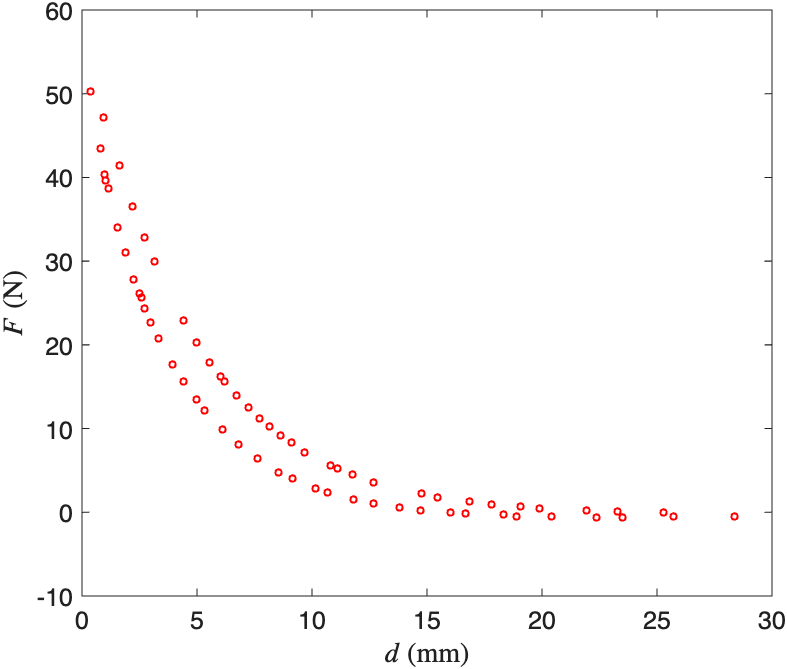
\includegraphics[width=7.5cm,height=5cm]{fig//ZFC}
                    \label{fig:0}
                    \caption{}
                \end{subfigure}
                \hfill
                \begin{subfigure}{0.45\textwidth}
                    \centering
                    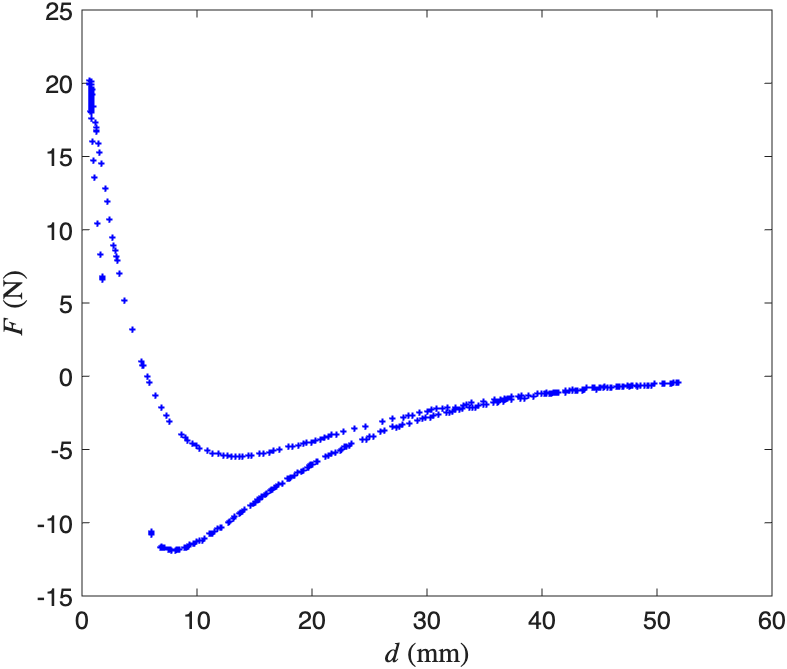
\includegraphics[width=7.5cm,height=5cm]{fig//FC}
                    \label{fig:1}
                    \caption{}
                \end{subfigure}
                \hfill
                \caption{(a)零场冷条件下磁悬浮力随距离的变化(b)场冷条件下磁悬浮力随距离的变化}
                \label{fig}
            \end{figure}
    \section{总结}
        本实验利用四引线法测量了超导体电阻以及温度计的读数，得到了超导体的超导转变曲线，此外还研究了零场冷和场冷条件下高温超导体与磁体之间的相互作用情况。
        通过对数据的进一步分析，我们确定了超导转变的临界温度。借助磁悬浮力与距离的定量关系，我们分析了非理想超导体的钉扎效应对超导体本身的影响。
    \begin{thebibliography}{99}
        \bibitem{1}
        北京师范大学物理实验教学中心. 近代物理实验讲义一 (2019)
    \end{thebibliography}

    
\end{document}